%%
%% Copyright 2007, 2008, 2009 Elsevier Ltd
%%
%% This file is part of the 'Elsarticle Bundle'.
%% ---------------------------------------------
%%
%% It may be distributed under the conditions of the LaTeX Project Public
%% License, either version 1.2 of this license or (at your option) any
%% later version.  The latest version of this license is in
%%    http://www.latex-project.org/lppl.txt
%% and version 1.2 or later is part of all distributions of LaTeX
%% version 1999/12/01 or later.
%%
%% The list of all files belonging to the 'Elsarticle Bundle' is
%% given in the file `manifest.txt'.
%%

%% Template article for Elsevier's document class `elsarticle'
%% with numbered style bibliographic references
%% SP 2008/03/01

\documentclass[preprint,1p]{elsarticle}
\biboptions{numbers,sort&compress}

%% Use the option review to obtain double line spacing
%% \documentclass[authoryear,preprint,review,12pt]{elsarticle}

%% Use the options 1p,twocolumn; 3p; 3p,twocolumn; 5p; or 5p,twocolumn
%% for a journal layout:
%% \documentclass[final,1p,times]{elsarticle}
%% \documentclass[final,1p,times,twocolumn]{elsarticle}
%% \documentclass[final,3p,times]{elsarticle}
%% \documentclass[final,3p,times,twocolumn]{elsarticle}
%% \documentclass[final,5p,times]{elsarticle}
%% \documentclass[final,5p,times,twocolumn]{elsarticle}

%% For including figures, graphicx.sty has been loaded in
%% elsarticle.cls. If you prefer to use the old commands
%% please give \usepackage{epsfig}

%% The amssymb package provides various useful mathematical symbols
\usepackage{amssymb}
\usepackage{lineno}
\usepackage{hyperref}
\usepackage{siunitx}
\usepackage{multirow}
\usepackage{wasysym}
\usepackage{tabularx}
\usepackage{mathtools}
%\usepackage[percent]{overpic}
%\usepackage[usenames,dvipsnames,svgnames,table]{xcolor}
%\usepackage{cleveref}

%% The amsthm package provides extended theorem environments
%% \usepackage{amsthm}

%% The lineno packages adds line numbers. Start line numbering with
%% \begin{linenumbers}, end it with \end{linenumbers}. Or switch it on
%% for the whole article with \linenumbers.
%% \usepackage{lineno}

\journal{Nucl. Instrum. Meth. A}

\begin{document}

\linenumbers

\begin{frontmatter}

%% Title, authors and addresses

%% use the tnoteref command within \title for footnotes;
%% use the tnotetext command for theassociated footnote;
%% use the fnref command within \author or \address for footnotes;
%% use the fntext command for theassociated footnote;
%% use the corref command within \author for corresponding author footnotes;
%% use the cortext command for theassociated footnote;
%% use the ead command for the email address,
%% and the form \ead[url] for the home page:
%% \title{Title\tnoteref{label1}}
%% \tnotetext[label1]{}
%% \author{Name\corref{cor1}\fnref{label2}}
%% \ead{email address}
%% \ead[url]{home page}
%% \fntext[label2]{}
%% \cortext[cor1]{}
%% \address{Address\fnref{label3}}
%% \fntext[label3]{}

\title{Simulation of the time resolution of a 50~$\mu$m low-gain avalanche detector.}

%% use optional labels to link authors explicitly to addresses:
%% \author[label1,label2]{}
%% \address[label1]{}
%% \address[label2]{}

\author[1,2]{C.~Pe\~na\corref{cor}}\ead{cmorgoth@fnal.gov}
\author[1]{G.~Deptuch}
\author[2]{S.~Xie}
\author[1]{A.~Apresyan}
\author[2]{L.~Narvaez}
\author[1]{T.~Liu}
\author[3]{N.~Cartiglia}


\address[1]{Fermi National Accelerator Laboratory, Batavia, IL, USA}
\address[2]{California Institute of Technology, Pasadena, CA, USA}
\address[3]{INFN, Torino, Italy}
\cortext[cor]{Corresponding author}

\begin{abstract}
%% Text of abstract
In this paper we report simulation results on the timing resolution of a 50~$\mu$m low-gain avalanche detector (LGAD).
The simulation includes: sensor fluctuations, front-end electronics, and quantization.
Comparisons on the performance for different front-end electonics (FEE) bandwidths (BWs) are presented, as well as
the dependance on singal-to-noise ratio (SNR).
Two approaches to measure the timestamp are presented: leading edge (LE) and constant-fraction-discrimination (CFD).
Aditionally, the time resolution is studied as function of the irradiation of the sensor.
Simulated LGAD pulses before irradiation, and after neutron fluences of
 $5\times 10^{14}$~n/cm$^2$ and $1\times 10^{15}$~n/cm$^2$, are studied.
 The time resolution a 50~$\mu$m LGADs was found to be ~30~ps for FE electronics BWs larger than 350~MHz and SNRs larger than 30.
 The time resolution at a SNR of 30 for fluences of $5\times 10^{14}$~n/cm$^2$ and $1\times 10^{15}$~n/cm$^2$ were found to be~30~\si{ps}
  and~40~\si{ps}, respectively.
\end{abstract}

\begin{keyword}
%% keywords here, in the form: keyword \sep keyword

%% PACS codes here, in the form: \PACS code \sep code
Silicon \sep Timing \sep LGAD
%% MSC codes here, in the form: \MSC code \sep code
%% or \MSC[2008] code \sep code (2000 is the default)

\end{keyword}

\end{frontmatter}

\tableofcontents

%% \linenumbers

%% main text
\section{Introduction}

Future colliders, including the high luminosity upgrade of the Large Hadron
Collider (HL-LHC) at CERN, will operate with an order of magnitude higher
instantaneous luminosity compared to what has been achieved at the
large hadron collider (LHC) so far.
With the increased instantaneous luminosity, the rate of simultaneous
interactions per bunch crossing (pileup) is projected to reach an average of 140
to 200. Pileup increases the difficulties in separating
particles from the hard scattering interaction with those
produced in different pileup interactions. In particular, the ability to discriminate between
jets produced in the events of interests, especially those associated with vector
boson fusion processes, and jets produced by pileup interactions will be
degraded. Additionally, the efficiency to identify high $p_{\mathrm{T}}$ isolated electrons
and muons will be severely reduced due to the high density of pileup particles
in their vicinity. The missing transverse energy resolution will also deteriorate, and several
other physics objects performance metrics will suffer the
detrimental effects of pileup.

One way to mitigate the pileup effects mentioned above, complementary to
precision tracking methods, is to perform a time of arrival measurement
associated with each particle. Such a measurement with a precision of about
30-40~\si{ps}, will reduce the effective amount of pileup by a factor of 10,
given that the spread in collision time of the pileup interactions at HL-LHC is
foreseen to be approximately 200~\si{ps}. It has been previously shown that a
precision of better than $20$~\si{ps} can be achieved for electromagnetic
showers measured with silicon sampling
calorimeters~\cite{Apresyan201662,Apresyan2017_NSSMIC,AKCHURIN201731} using
traditional planar silicon detectors while precision of $30$~\si{ps} can be achived for minimum ionizing particles (MIPs) measured
with low-gain avalanches detectors (LGADs) ~\cite{Apresyan:2018oln, Cartiglia201783, PELLEGRINI201412}.

LGADs are envisioned to be used in the CMS and ATLAS experiment upgrades for HL-LHC in order to overcome
the event reconstruction challenges posed by the high rate of concurrent
collisions per beam crossing. The implemented regions of pseudorapidity ($\eta$)
are: $|\eta|>1.5$, and $2.4 < |\eta| < 4.2 $ for CMS and ATLAS, respectively. In
order to achieve the desired timing precision across a large area of the
detectors, the sensors will need to provide high uniformity of signal response
and timing resolution. Beam test measurements have provided encouraging results towards achieving
such detectors~\cite{Apresyan:2018oln}.

In this paper, we report simulation results on the
timing resolution of a 50~$\mu$m low-gain avalanche detector (LGAD) which includes
the effects of the sensor fluctuations, front-end electronics (FEE), and quantization.
Our results indicate that for FEE analog bandwidths (BWs) larger than 350 MHz and signal-to-noise ratios
(SNRs) larger than 30, measured at the output of the FFE, time resolutions of $30$~\si{ps} and $40$~\si{ps}
are obtained when using time-walk corrections based on time-over-therhold (ToT)
measurements to both timestamping techniques: constand-fraction-dricrimination (CFD) and leading-edge (LE), respectively. These results are
compatible with previous measurements on LGAD timing resolutions carried out in laboratory and beam test
conditions~\cite{Apresyan:2018oln, Cartiglia201783, PELLEGRINI201412}. We study the time resolution for four
different FEE shaping times: $0.5$~\si{ps}, $1.0$~\si{ps}, $2.0$~\si{ps}, and $4.0$~\si{ps}; three SNR: 20, 30, 100; and three
irradiation levels: pre-radiation, $5\times 10^{14}$~n/cm$^2$, and $1\times 10^{15}$~n/cm$^2$. For every point in this scan we
 evaluate the time resolution for LE and CFD.

The paper is organized as follows: the simulation is described in
Sec.~\ref{sec:simulation}; algorithms used in the timing
reconstruction and analysis are described in Sec.~\ref{sec:timing_and_analysis}; simulation results
are presented in Sec.~\ref{sec:results}, followed by the conclusion in
Sec.~\ref{sec:conclusion}.

\section{Simulation Framework}
\label{sec:simulation}

%We performed the test-beam measurements at the Fermilab Test-beam
%Facility%

The simulation framework is based on c++ programing language. The LGAD pulses are obtained
from Weightfield2 (WF2), a 2-dimensional silicon simulator~\cite{WF2}. WF2 provides sets of 1000 LGAD pulses which models the response
of the sensor to minimum ionizing particles (MIPs). We generated 3 sets of LGAD pulses for a 50~$\mu$m LGAD:
 pre-irradiation, and after neutron fluences of $5\times 10^{14}$~n/cm$^2$ and $1\times 10^{15}$~n/cm$^2$. The simulation framework
 takes the LGAD pulses (from WF2) and adds gaussian white noise (hereafter white noise). At this point the LGAD pulses with the added white noise
 are fed into the simulation of the FEE (see Fig.~\ref{fig:simulation_diagram}). The output of the FEE simulation is the convolution of the
 impulse response function and the input signal at the FEE. We consider four shaping constants for the impulse response
 of the FEE: 0.5, 1.0, 2.0, and 4.0~\si{ns} (the FEE simulation will be described in detail
 in Sec.~\ref{sub_sec:fee_simulation_and_noise}). At the output of the FEE block we have a "realistic" LGAD pulse which includes the effects
 of sensor fluctuations, shaping of the FEE, and noise. A waveform analysis is performed
  with the pulses obtained at the output of the FEE block. We assign timestamps to each pulse by using algorithms that emulate
  an ideal LE discriminator and an ideal CFD. For each threhold we obtain a LE and CFD
  timestamps as well as the corresponding time-over-theshold (ToT) of the pulse.
  The SNR is defined as the ratio of the most probable value (MPV) of the amplitude distribution to the
  width of the amplitude distribution at a fixed sample (where only noise is present). We study 3 SNR scenarios: 20, 30, and 100.
  A schematic diagram of the simulation is shown in Fig.~\ref{fig:simulation_diagram}.

\begin{figure}[htbp]
\centering
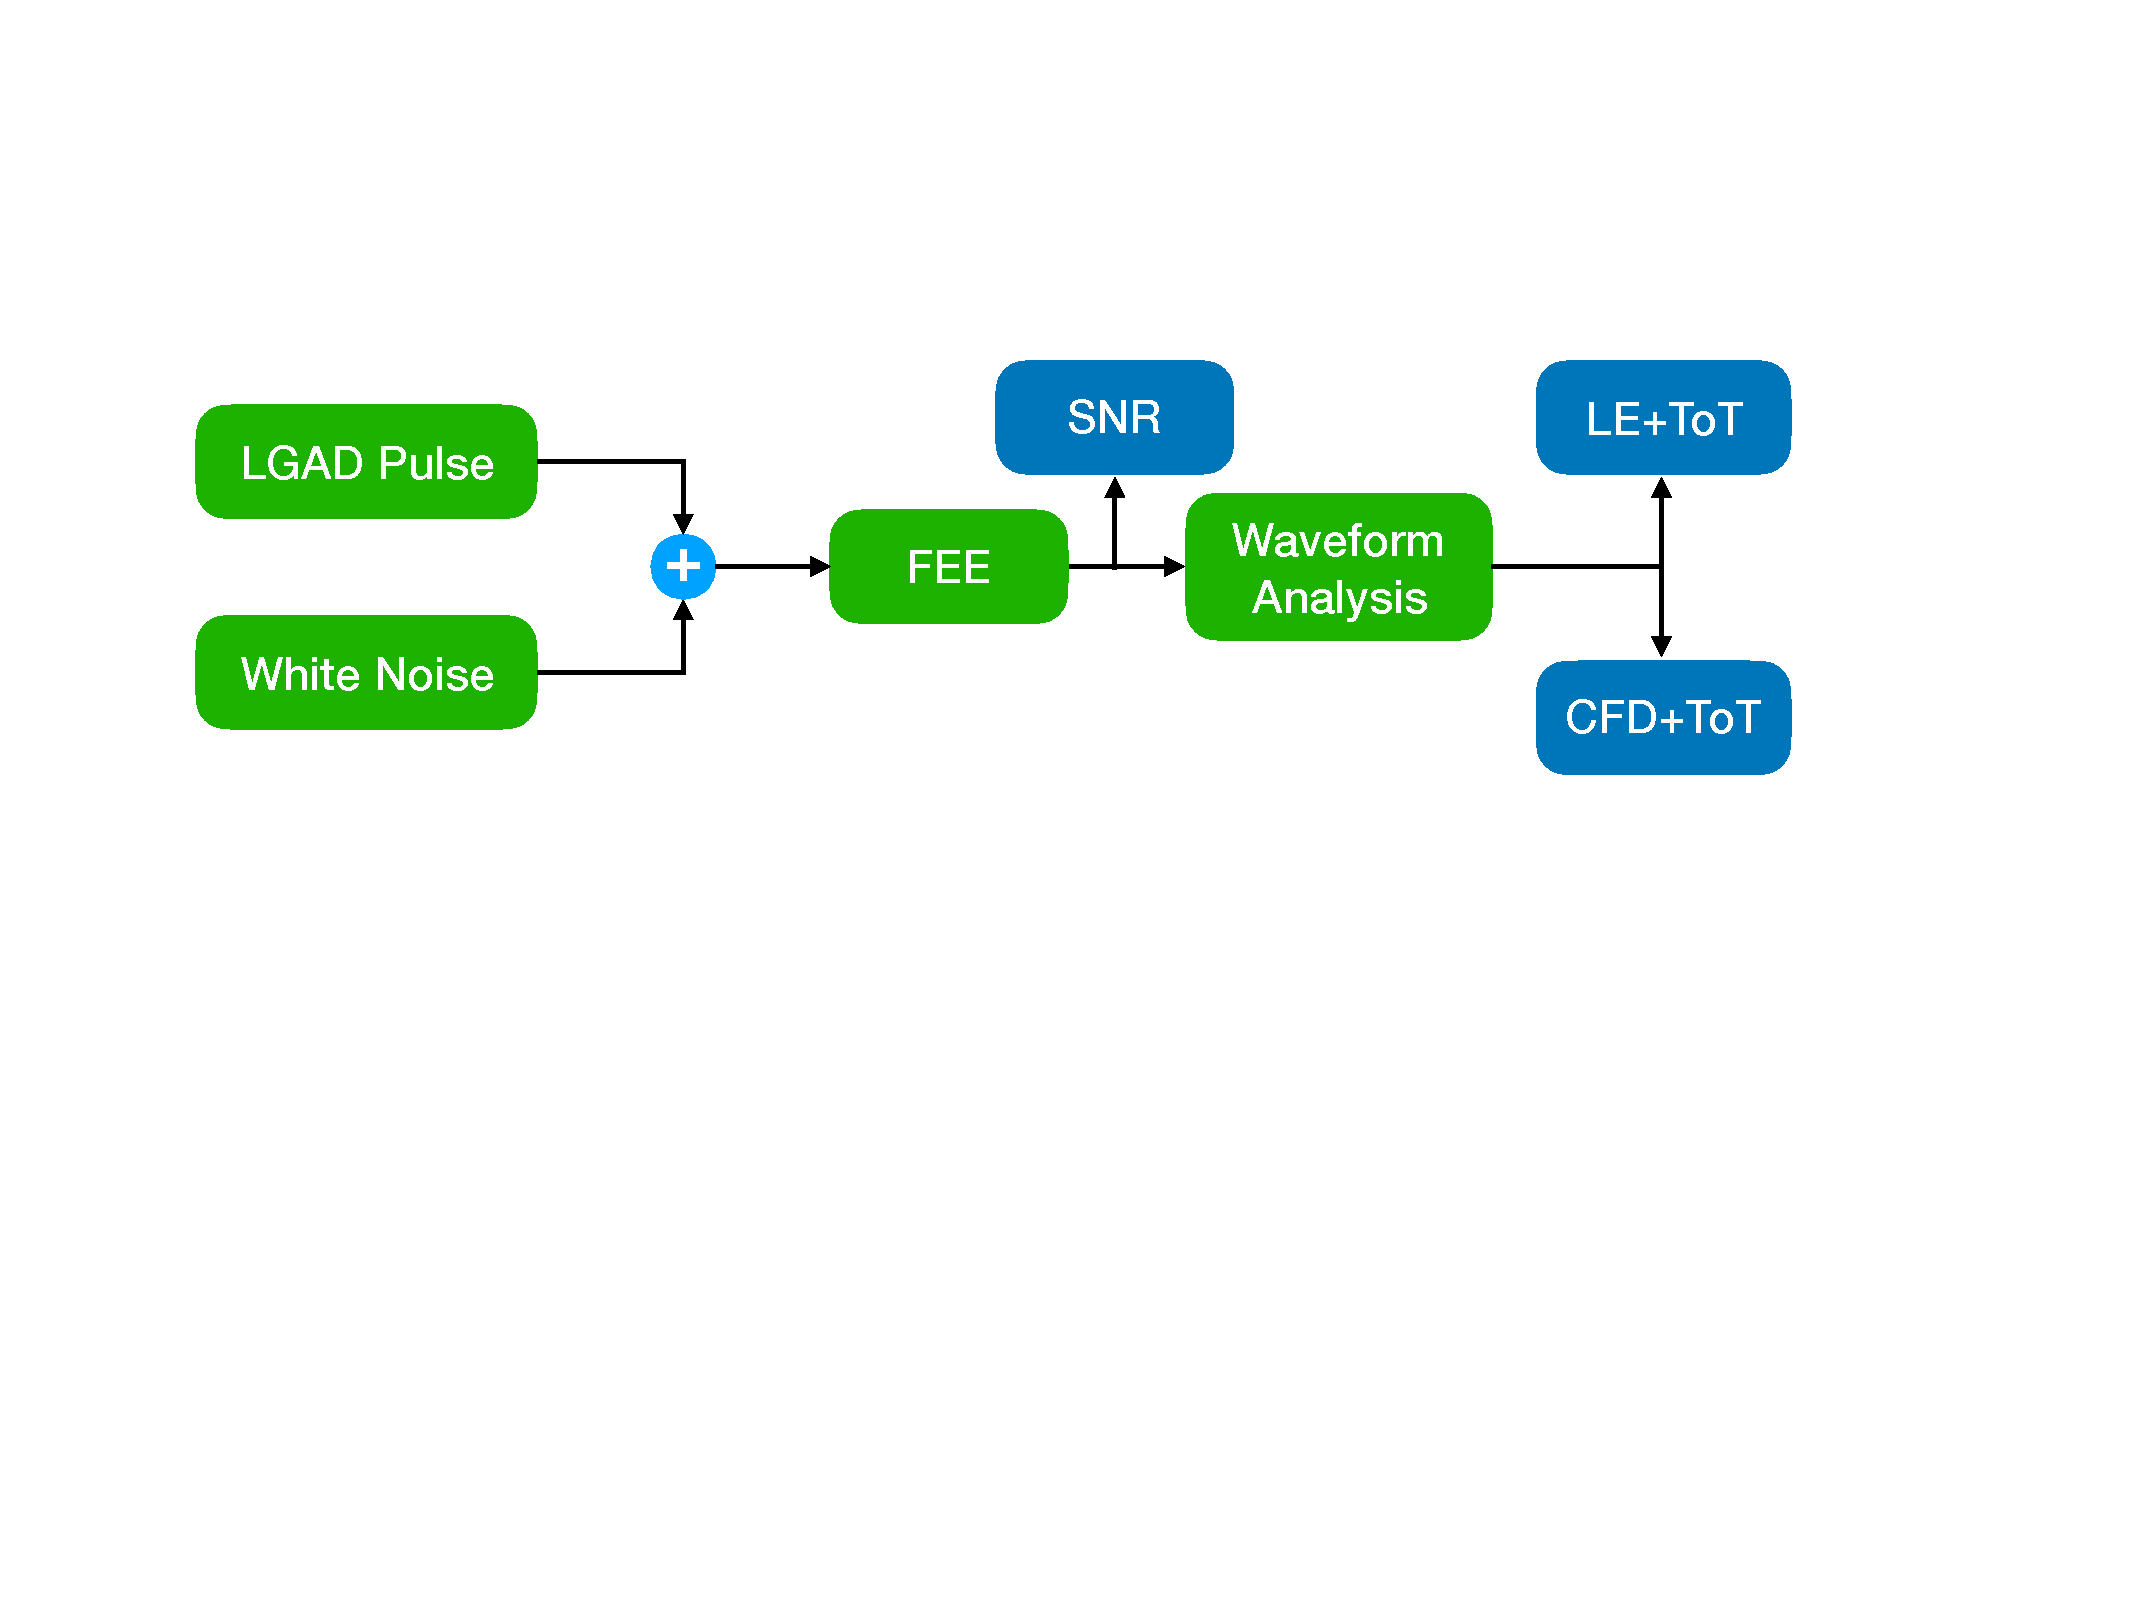
\includegraphics[width=0.75\textwidth]{figs/lgad_simulation_diagram.pdf}
\caption{A schematic diagram of the simulation. Each simulation configurable block is shown in green. The most relevant outputs
of the simulation are shown in blue.}
\label{fig:simulation_diagram}
\end{figure}

\subsection{LGAD pulse library and simulation}
\label{sub_sec:lgad_pulse_library}
We need to ask Nicolo to send us a paragrah for the Weightfield2 (WF2)

\subsection{Fron-end Electronics simulation and noise injection}
\label{sub_sec:fee_simulation_and_noise}
The front-end simulation is implemented in c++ programing language. It combines analytical calculations when possible but
it mostly relies on numerical methods. We implement most calculations in the time domain, while the frequency domain is mostly used
to cross-check noise and the FEE expected response. Sections~\ref{sec:fee} and~\ref{sec:noise_simulation} detail the front-end and
noise implementation in the simulation.

\subsubsection{front-end implementation}\label{sec:fee}
The fron-end simulation is based on a single amplification stage. We focus on the BW of such amplifier rather than variations
thereof. The fron-end chose is a second order low-pass filter which transfer function
and impulse response are given by equations~\ref{eq:filter_tf} and~\ref{eq:filter_ir}, respectively.


 \begin{tabularx}{\textwidth}{XX}
 \begin{equation}\label{eq:filter_tf}
   H(S) = \frac{\frac{1}{\tau_{s}^{2}}}{(S+1/\tau_{s})^{2}}
 \end{equation}
     &
 \begin{equation}\label{eq:filter_ir}
     h(t) = \frac{t}{\tau_s^2}e^{-t/\tau_{s}}
 \end{equation}
 \end{tabularx}\par

 The output pulse of the FEE is the convolution (in time domain) of the pulse from the LGAD library and the FEE impulse response
 (see Eq.~\ref{eq:filter_ir}).
 The time base for the pulses and the convolution is 10~\si{ps} -- this sampling time is used throughout the simulation. As stated above we focus the study
 on the BW of the FEE, to that end we scan the $\tau_{s}$ paremeter in Eq.~\ref{eq:filter_ir} in the following set:\{0.5, 1, 2, 4\}~\si{ns}, this parameter is hereafter referred to as
 shaping time (ST). Figure~\ref{fig:ir_and_lgad} (left) shows the comparison of the impulse and LGAD responses for a ST of 1~\si{ns} while
 Figure~\ref{fig:ir_and_lgad} (right) shows the LGAD response for all STs studied. We obseve that the LGAD response is delayed with respect
 to the impulse response,  and that pulse slew rate is decreased in the first nanosecond of the pulse. We also observe the expected
 behavior when comparing the LGAD responses for the different STs, pulse risetimes scale with the ST and the decay time is dominated by
 the ST.


\begin{figure}[htbp]
  \centering
  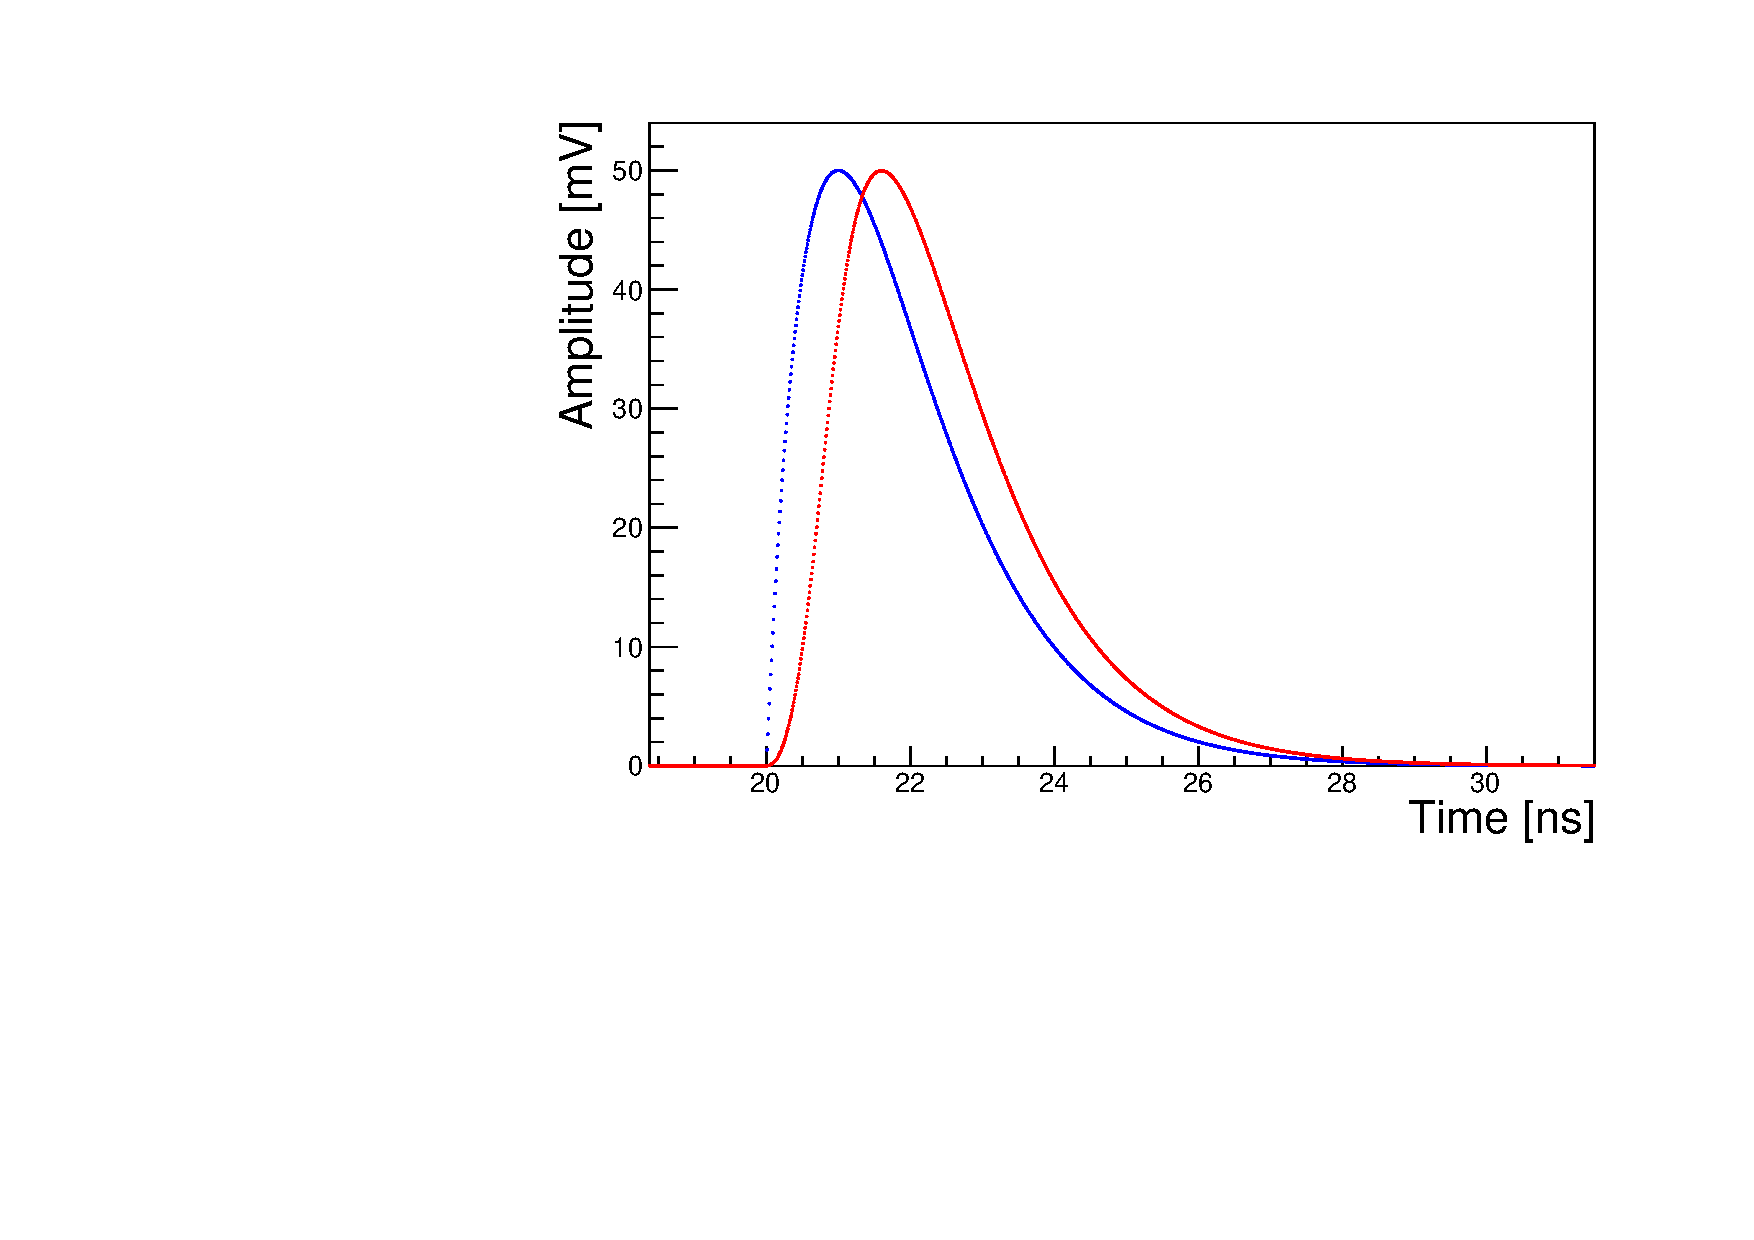
\includegraphics[width=0.48\textwidth]{figs/impulse_vs_lgad_response_1ens_shaping.pdf} \hfill
  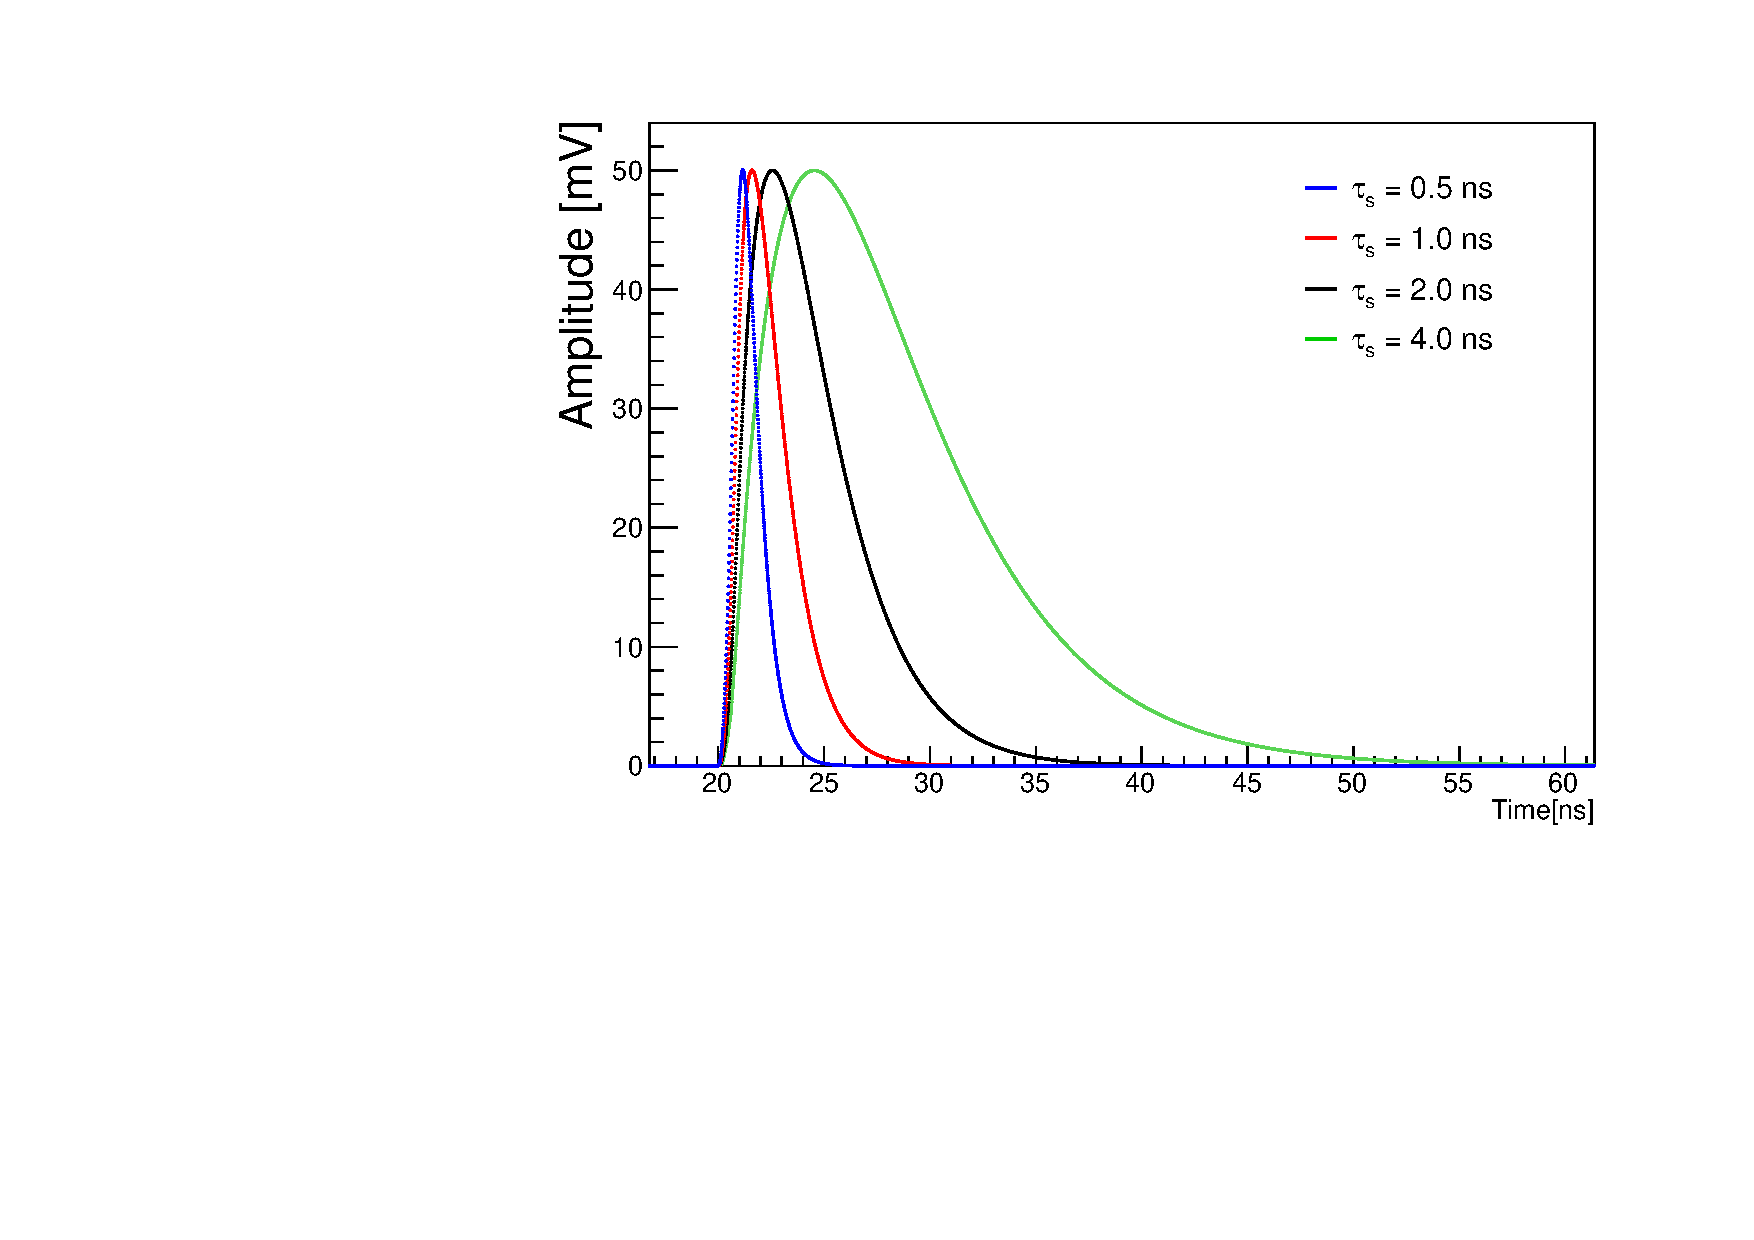
\includegraphics[width=0.48\textwidth]{figs/lgad_all_shaping_time_noiseless.pdf}
  \caption{(Left) Comparison of impulse and LGAD reponses for the a shaping time (ST) of 1~\si{ns}.
  (Right) LGAD response for the four shaping times studied: \{0.5, 1, 2, 4\}~\si{ns}. All pulses have been nomalized
  to achive a peak amplitude of 50~\si{mV}. Legends for the shaping times are shown in the plots.}
  \label{fig:ir_and_lgad}
\end{figure}

\begin{table}[!htb]
\scriptsize
\begin{center}
  \begin{tabular}{ |c | c | c | c | c | }
    \hline
    Shaping time (ns) & 0.5         & 1.0         & 2.0         & 4.0 \\ \hline
    Risetime (ns)     & $0.7\pm xx$ & $0.9\pm xx$ & $1.4\pm xx$ & $2.5\pm xx$ \\
    \hline
  \end{tabular}
\caption{Measured risetime for all shaping times studied: \{0.5, 1, 2, 4\}~\si{ns}. Risetime is the $10\% - 90\%$ time
difference as measured by the CFD algorithm described in Sec.~\ref{sec:le_and_cfd}.}
\label{tab:sensors}
\end{center}
\end{table}


\subsubsection{noise injection}\label{sec:noise_simulation}
Gaussian white noise is simulated by sampling the full time window (0 - 100~\si{ns}) in 10~\si{ps} intervals. At each
sampled time we assign a random amplitude which is drawn from from a gaussian distribution with zero mean and with corresponding to the SNR
under study. It is important to note that the width of the gausian parameter is not exactly the SNR and needs to be adjusted depending
on the ST of the FEE under study.
\section{Timing Reconstruction and Analysis}
\label{sec:timing_and_analysis}

\subsection{Leading edge and constant fraction discriminators}
\label{sec:le_and_cfd}

\subsection{Time-walk correction and time over threshold}
\label{sec:tw_and_tot}

% \begin{figure}[!htbp]
% \centering
% \includegraphics[width=0.3\textwidth]{figs/HPK-50D-PIX.pdf}
% \includegraphics[width=0.31\textwidth]{figs/Hgtd_Hg11_a.jpg} \\
% \includegraphics[width=0.32\textwidth]{figs/HPK-50D-GR.pdf}
% \includegraphics[width=0.31\textwidth]{figs/Lgad_Lga35_a.jpg}
% \caption{Photographs of the HPK 50D-PIX $2\times 2$ array sensor (top left), the CNM W9HG11 $2\times 2$
% array sensor (top right), the HPK 50D-GR single sensor (bottom left), and the CNM W11LGA35 single
% sensor (bottom right) are shown. Numerical labels overlaid on top of the images of the array sensors are
% used in the text when referring to individual pixels.}
% \label{fig:HPK_Sensors}
% \end{figure}

% \begin{table}[!htb]
% \scriptsize
% \begin{center}
%   \begin{tabular}{ |c | c | c | c | }
%     \hline
%     Sensor      & Number of channels & Single channel dimensions &  Single channel capacitance  \\ \hline
%     HPK 50A-PIX & 4 & $3\times 3$~$\mathrm{mm}^{2}$ & 20 pF \\
%     HPK 50B-PIX & 4 & $3\times 3$~$\mathrm{mm}^{2}$ & 20 pF \\
%     HPK 50C-PIX & 4 & $3\times 3$~$\mathrm{mm}^{2}$ & 20 pF \\
%     HPK 50D-PIX & 4 & $3\times 3$~$\mathrm{mm}^{2}$ & 20 pF \\
%     HPK 80C-PIX & 4 & $3\times 3$~$\mathrm{mm}^{2}$ & 12 pF \\
%     HPK 50D     & 1 & $\diameter=1.0$~$\mathrm{mm}$  & 2.9 pF \\
%     CNM-W9HG11  & 4 & $3\times 3$~$\mathrm{mm}^{2}$ & 22 pF \\
%     CNM-W11LGA35& 1 & $1.3\times 1.3$~$\mathrm{mm}^{2}$ & 3.9 pF \\
%     \hline
%   \end{tabular}
% \caption{Linear dimensions and capacitances of the sensors used in these studies.}
% \label{tab:sensors}
% \end{center}
% \end{table}



%\begin{table}[!htb]
%	\tiny
%	\begin{center}
%		\begin{tabular}{ |c | c | c| c | }
%			\hline
%			Sensor      & KU Board 2-ch & UCSC board 4-ch & FNAL board 4-ch \\ \hline \hline
%			HPK 50A-PIX & \textbf{-630 V (13)} & -- & -- \\ \hline
%			HPK 50B-PIX & \begin{tabular}{@{}c@{}}\textbf{-450 V (10), -550 V (25), -600 V (60)}\\ \underline{-510 V} \\ \textit{-510 V, -570 V}\end{tabular}  & -- & -- \\ \hline
%			HPK 50C-PIX & \textbf{-400 V (20)} & \textbf{-410 V (22), -470 V (40)} & -- \\ \hline
%			HPK 50D-PIX & \begin{tabular}{@{}c@{}}\textbf{-100 V (7), -200V (11),} \\ \textbf{ -250 V (17), -300 V (30), } \\ \textbf{-325 V (40)}\end{tabular}  & -- & \begin{tabular}{@{}c@{}}\textbf{-250 V (17), -300 V (30),} \\ \underline{-210 V, -250 V} \\ \textit{-250 V (30), -280 V (40)}\end{tabular} \\ \hline
%			CNM W9HG11 & -- & \textbf{-140 V (10), -160 V (12), -180 V (14)} & -- \\ \hline
%			\begin{tabular}{@{}c@{}}HPK 50D \\  $6\times 10^{14}$~n/cm$^2$ \end{tabular} & -- & \textit{-600 V (20), -635 V (30)} & -- \\ \hline
%			\begin{tabular}{@{}c@{}}CNM W11LGA35 \\ $6\times 10^{14}$~n/cm$^2$ \end{tabular} & -- & -- & \textit{-400 V (24), -420 V (28)} \\ \hline
%			\hline
%		\end{tabular}
%		\caption{Data taking conditions for the studies presented in this paper. Numbers in bold indicate that the sensor was at  room temperature, underlined ones were taken at $-10$C$^{\circ}$, and those in italicized text were taken at $-20$C$^{\circ}$.}
%		\label{tab:DataConditions}
%	\end{center}
%\end{table}
%

% \begin{table}[!htb]
% 	\tiny
% 	\begin{center}
% 		\begin{tabular}{ |c | c | c| c | }
% 			\hline
% 			Sensor      & KU Board 2-ch & UCSC board 4-ch & FNAL board 4-ch \\ \hline \hline
% 			HPK 50A-PIX & \textbf{-630 V (20)} & -- & -- \\ \hline
% 			HPK 50B-PIX & \begin{tabular}{@{}c@{}}\textbf{-550 V (25)}\end{tabular}  & -- & -- \\ \hline
% 			HPK 50C-PIX & \begin{tabular}{@{}c@{}}\textbf{-400 V (20)}\end{tabular} & \textbf{ -450 V (35)} & -- \\ \hline
% 			HPK 50D-PIX & \begin{tabular}{@{}c@{}}\textbf{-300 V (30)} \end{tabular}  & -- & \begin{tabular}{@{}c@{}}\textbf{-250 V (17), -300 V (30),} \\ \underline{-250 V (29)} \\ \textit{-250 V (36)}\end{tabular} \\ \hline
% 			CNM W9HG11 & -- & \textbf{-180 V (14)} & -- \\ \hline
% 			\begin{tabular}{@{}c@{}}HPK 50D \\  $6\times 10^{14}$~n/cm$^2$ \end{tabular} & -- & \textit{-600 V (20), -635 V (30)} & -- \\ \hline
% 			\begin{tabular}{@{}c@{}}CNM W11LGA35 \\ $6\times 10^{14}$~n/cm$^2$ \end{tabular} &
% 			-- & \textit{-400 V (24), -420 V (28)}  & --\\ \hline
% 		\end{tabular}
% 		\caption{Data taking conditions for the studies presented in this paper. Numbers in bold indicate that the sensor was at room temperature, underlined ones were taken at $-10$C$^{\circ}$,
% 		  and those in italicized text were taken at $-20$C$^{\circ}$. The numbers in parenthesis indicate the gain at the given operation voltage. }
% 		\label{tab:DataConditions}
% 	\end{center}
% \end{table}


\section{LGAD Front-end Electronics Performance}
\label{sec:results}

We present a number of different studies of the LGAD sensors.
such that they are above the noise levels listed for each board in
Sec.~\ref{sec:boards}. All measurements other than those described in
Sec.~\ref{sec:temp_dependance} and ~\ref{sec:rad_tolerance} were performed at
room temperature.
\subsection{Front-end electronics shaping time studies}
\label{sec:shaping_time}
\subsection{Timing Performace as a function of signal-to-noise ratio}
\label{sec:snr}
\subsection{Timing Performace as a function of irradiation}
\label{sec:rad_tolerance}



% \begin{figure}[htbp]
% \centering
% \includegraphics[width=0.48\textwidth]{figs/USCSBoard_HPK50DIrradiated-CNMW11LGA35_Run936-961/CNM_irradiated_amp_Map.pdf} \hfill
% \includegraphics[width=0.48\textwidth]{figs/USCSBoard_HPK50DIrradiated-CNMW11LGA35_Run936-961/CNM_irradiated_amp_1D.pdf}
% \caption{(Left) The map of the amplitude distribution on the irradiated CNM W11LGA35 sensor across X and Y coordinates. Two distinct regions on the sensor surface can be identified according to the amplitude distribution: the center of the sensor (area within the red circle), and the periphery of the sensor (area between the black circle and black square). (Right) Amplitude distribution in the two areas of the irradiated CNM W11LGA35 sensor. The sensor was irradiated to $6\times 10^{14}$~n/cm$^2$. Measurements were performed at $-20^{\circ}$C.}
% \label{fig:CNM_irradiated_amp_Map}
% \end{figure}


% \begin{figure}[htbp]
% \centering
% \includegraphics[width=0.48\textwidth]{figs/USCSBoard_HPK50DIrradiated-CNMW11LGA35_Run936-961/HPK_irradiated_amp_Map.pdf} \hfill
% \includegraphics[width=0.48\textwidth]{figs/USCSBoard_HPK50DIrradiated-CNMW11LGA35_Run936-961/HPK_irradiated_amp_1D.pdf}
% \caption{(Left) The map of the amplitude distribution on the irradiated HPK 50D sensor across X and Y coordinates. (Right) Signal amplitude distribution for the irradiated HPK 50D sensor. The sensor was irradiated to $6\times 10^{14}$~n/cm$^2$. Measurements were performed at $-20^{\circ}$C.}
% \label{fig:HPK_irradiated_amp_Map}
% \end{figure}



% \begin{figure}[htbp]
% \centering
% \includegraphics[width=0.90\textwidth]{figs/USCSBoard_HPK50DIrradiated-CNMW11LGA35_Run936-961/IrradiatedSensorStudy_Efficiency_vs_X.pdf}
% \includegraphics[width=0.90\textwidth]{figs/USCSBoard_HPK50DIrradiated-CNMW11LGA35_Run936-961/IrradiatedSensorStudy_Efficiency_vs_Y.pdf}
% \caption{Efficiency measurements across the X-axis (top) and Y-axes (bottom) of the HPK 50D and CNM W11LGA35 irradiated sensors. Both sensors were irradiated to $6\times 10^{14}$~n/cm$^2$. Measurements were performed at $-20^{\circ}$C.}
% \label{fig:IrradiatedSensorStudy_Efficiency}
% \end{figure}


% \begin{figure}[htbp]
% \centering
% \includegraphics[width=0.90\textwidth]{figs/USCSBoard_HPK50DIrradiated-CNMW11LGA35_Run936-961/IrradiatedSensorStudy_MPV_vs_X.pdf}
% \includegraphics[width=0.90\textwidth]{figs/USCSBoard_HPK50DIrradiated-CNMW11LGA35_Run936-961/IrradiatedSensorStudy_MPV_vs_Y.pdf}
% \caption{Signal amplitude MPV measurement across the X-axis (top) and Y-axes (bottom) of the HPK 50D and CNM W11LGA35 irradiated sensors. Both sensors were irradiated to $6\times 10^{14}$~n/cm$^2$. Measurements were performed at $-20^{\circ}$C.}
% \label{fig:IrradiatedSensorStudy_MPV}
% \end{figure}




% \begin{figure}[htbp]
% \centering
% \includegraphics[width=0.9\textwidth]{figs/USCSBoard_HPK50DIrradiated-CNMW11LGA35_Run936-961/IrradiatedSensorStudy_MeanTime_vs_X.pdf}
% \includegraphics[width=0.9\textwidth]{figs/USCSBoard_HPK50DIrradiated-CNMW11LGA35_Run936-961/IrradiatedSensorStudy_MeanTime_vs_Y.pdf}
% \caption{$\Delta{t}$ measurements across the X-axis (top) and Y-axes (bottom) of the HPK 50D and CNM W11LGA35 irradiated sensors. Both sensors were irradiated to $6\times 10^{14}$~n/cm$^2$. Measurements were performed at $-20^{\circ}$C.}
% \label{fig:IrradiatedSensorStudy_MeanTime}
% \end{figure}


% \begin{figure}[htbp]
% \centering
% \includegraphics[width=0.90\textwidth]{figs/USCSBoard_HPK50DIrradiated-CNMW11LGA35_Run936-961/IrradiatedSensorStudy_TimeResolution_vs_X.pdf}
% \includegraphics[width=0.90\textwidth]{figs/USCSBoard_HPK50DIrradiated-CNMW11LGA35_Run936-961/IrradiatedSensorStudy_TimeResolution_vs_Y.pdf}
% \caption{Time resolution measurements across the X-axis (top) and Y-axes (bottom) of the HPK 50D and CNM W11LGA35 irradiated sensors. Both sensors were irradiated to $6\times 10^{14}$~n/cm$^2$. Measurements were performed at $-20^{\circ}$C.}
% \label{fig:IrradiatedSensorStudy_TimeResolution}
% \end{figure}



\section{Conclusion}
\label{sec:conclusion}

% In a beam test at FNAL with tracking information, we compared the performance of
% LGAD produced by CNM Barcelona and HPK Hamamatsu. Single pads of diameter 1~mm
% and $2\times 2$ arrays of square pixels of 3~mm were used. Sensors with
% thicknesses of about 50 and 80 $\mu$m were studied. The uniformity of the
% sensor response in pulse height, efficiency, and timing resolution
% were studied. Four different readout boards
% were used in these studies. The uniformity of the
% sensor response in pulse height before irradiation was found to have a
% 2\% spread. The efficiency and timing  resolution before irradiation
% were found to be 100\%  and 30-40~\si{ps}, respectively. The
% ``non-response'' region between pixels was measured to be about 130~$\mu$m for CNM sensors
% and 170~$\mu$m for HPK sensors.
% A small timing shift across the HPK sensor of the order 20--30~\si{ps} can
% be explained by the observed change in pulse shape when comparing metalized and
% non-metalized sensor areas. Uniform signal detection efficiency of 100\% is
% observed on all sensors, both before and after irradiation.
%
% For an un-irradiated 50~$\mu$m thick LGADs with 3~mm pads we find the following timing results:
% \begin{itemize}
%   \item at a temperature of $+20^{\circ}$C, the timing resolution ranges from
%         40~ps to 50~ps depending on the readout board. %This number worsens by
%         %10~ps for a 80~$\mu$m sensor.
%         %This last statement is not true
%   \item cooling the LGAD, while keeping the bias voltage the same at $-250$~V,
%         improves the timing resolution from 55~ps at $+20^{\circ}$C to 43~ps at
%         $-10^{\circ}$C to 36 ps at $-20^{\circ}$C. \end{itemize}
%
% After a neutron fluence of $6\times 10^{14}$~n/cm$^2$, the single pad CNM sensor
% exhibits a large gain variation of a factor 2.5 when comparing metalized and
% non-metalized sensor areas. For an 50~$\mu$m thick LGAD with 1~mm pads
% irradiated $6\times 10^{14}$~n/cm$^2$ we find the following timing results when
% operated at $-20^{\circ}$C:
%
% \begin{itemize}
%   \item for the HPK LGAD the highest bias voltage reached is $-635$~V
%     and the corresponding timing resolution is 30~ps;
%   \item for the CNM LGAD the highest bias voltage reached is $-420$~V
%     and the corresponding
%         timing resolution is 30~ps for the metalized area and $40$~ps for the
%         non-metalized area.
% \end{itemize}

\section*{Acknowledgment}

We thank the FTBF personnel and Fermilab accelerator's team for very good beam
conditions during our test beam time. We also appreciate the technical support
of the Fermilab SiDet department for the rapid production of wire-bonded and
packaged LGAD assemblies. We would like to thank Alan Prosser and Ryan Rivera
for their critical help in setting up the DAQ and trigger chain. We thank Ned
Spencer, Max Wilder, and Forest McKinney-Martinez for their technical
assistance, and the CNM and HPK manufacturing team. We acknowledge the help of
V. Cindro and I. Mandic with the neutron irradiations.

This document was prepared using the resources of the Fermi National Accelerator
Laboratory (Fermilab), a U.S. Department of Energy, Office of Science, HEP User
Facility. Fermilab is managed by Fermi Research Alliance, LLC (FRA), acting
under Contract No. DE-AC02-07CH11359. Part of this work was performed within the
framework of the CERN RD50 collaboration.

This work was supported by the Fermilab LDRD 2017.027; by the United States
Department of Energy grant DE-FG02-04ER41286; by the California Institute of
Technology High Energy Physics under Contract DE-SC0011925; by the European
Union's Horizon 2020 Research and Innovation funding program, under Grant
Agreement no. 654168 (AIDA-2020) and Grant Agreement no. 669529 (ERC
UFSD669529); by the Italian Ministero degli Affari Esteri and INFN Gruppo V; and
by the Spanish Ministry of Economy, Industry and Competitiveness through the
Particle Physics National Program (ref. FPA2014-55295-C3-2-R and
FPA2015-69260-C3-3-R) co-financed with FEDER funds.


% The Appendices part is started with the command \appendix;
% appendix sections are then done as normal sections

%\appendix
%\section{Appendix A}



% \section{}
% \label{}

%% If you have bibdatabase file and want bibtex to generate the
%% bibitems, please use
%%
%%  \bibliographystyle{elsarticle-num}
%%  \bibliography{<your bibdatabase>}

%% else use the following coding to input the bibitems directly in the
%% TeX file.

\bibliography{lgad_frontend_simulation}{}
\bibliographystyle{ieeetr}

%\begin{thebibliography}{00}

%% \bibitem{label}
%% Text of bibliographic item

%\bibitem{}

%\end{thebibliography}
\end{document}
\endinput
%%
%% End of file `elsarticle-template-num.tex'.
